\documentclass{article}

\usepackage{../../preamble}

\title{PGM: Homework 1}
\author{Raphael Reme}

\begin{document}
\maketitle
\section{Linear classification}
\subsection{Generative model (LDA)}
Given the class variable, the data are assumed to be Gaussian with different means for different classes but with the same covariance matrix.
\begin{equation*}
    y \sim \mathcal{B}(\Pi), x | y=i \sim \mathcal{N}(\mu_i, \Sigma)
\end{equation*}


\paragraph{a.} Derive the form of the maximum likelihood estimator for this model.\\
\vspace{5px}\\
Let $\set{(X_k, Y_k)}_{k \in \Inter{1}{n}}$ iid random variables. Such that $Y_k \sim \mathcal{B}(\Pi)$ and $X_k | Y_k=i \sim \mathcal{N}(\mu_i, \Sigma)$. (Note that $\Pi$
is the parameter and that I will use $\pi$ as the numerical value pi.) Let's call ${(x_k, y_k)}_{k \in \Inter{1}{n}}$ a realisation of these variables.
And $X = \begin{pmatrix} x_1^T \\ \vdots \\ x_n^T \end{pmatrix} \in \R^{n \times d}, Y = \begin{pmatrix} y_1 \\ \vdots \\ y_n \end{pmatrix} \in \R^n$. Our
goal is to estimate the parameter $\theta = (\Pi, \mu_0, \mu_1, \Sigma)$ with the maximization of the (log-)likelyhood:
\begin{equation*}
    \begin{aligned}
        L_{X, Y}(\theta) & = \log p(X, Y | \theta)                                                         &                                       \\
                         & = \log \prod_k p(x_k, y_k | \theta)                                             & \text{(Independence of $(X_k, Y_k)$)} \\
                         & = \sum_k \log p(y_k | \theta)  + \log p(x_k | Y_k=y_k, \theta)                  &                                       \\
                         & = \sum_k \log \mathcal{B}(y_k; \Pi)  + \log \mathcal{N}(x_k; \mu_{y_k}, \Sigma) &                                       \\
    \end{aligned}
\end{equation*}\\
In order to simplfy the expression we can introduce the partition
$P \cup Q = \Inter{1}{n}$ such that $\forall p \in P, y_p=1$ and $\forall q \in Q, y_q=0$. Let's call $N = \#P$.
(I will suppose that there is at least one example of each classes: $N \in \Inter{1}{n-1}$)

\begin{equation*}
    \begin{aligned}
        L_{X, Y}(\theta) & = \sum_{p \in P} \log \mathcal{B}(1; \Pi) + \sum_{q \in Q} \log \mathcal{B}(0; \Pi) + \sum_{p \in P} \log \mathcal{N}(x_p; \mu_1, \Sigma) + \sum_{q \in Q} \log \mathcal{N}(x_q; \mu_0, \Sigma) &                                              \\
                         & \begin{aligned}
             & = N\log(\Pi) + (n - N)\log(1-\Pi) - \frac{nd}{2}\log(2\pi) - \frac{n}{2}\log(|\Sigma|)                                                      \\
             & \;\;- \frac{1}{2}\sum_{p \in P} (x_p - \mu_1)^T\Sigma^{-1}(x_p - \mu_1) - \frac{1}{2}\sum_{q \in Q} (x_q - \mu_0)^T\Sigma^{-1}(x_q - \mu_0)
        \end{aligned}                                                                                                                                                                       & \text{($\Sigma \in S^d_{++}$ by definition)} \\
    \end{aligned}
\end{equation*}\\
$\widehat{\theta} = (\widehat\Pi, \widehat\mu_0, \widehat\mu_1, \widehat\Sigma)$ is an extremum point of the likelyhood which is a differentiable function. Therefore it verifies:

\begin{equation*}
    \nabla_\theta L_(X, Y)(\widehat\theta) = 0 \Leftrightarrow \begin{aligned}
         & \nabla_\Pi L_(X, Y)(\widehat\theta) = 0      & (1) \\
         & \nabla_{\mu_0} L_(X, Y)(\widehat\theta) = 0  & (2) \\
         & \nabla_{\mu_1} L_(X, Y)(\widehat\theta) = 0  & (3) \\
         & \nabla_{\Sigma} L_(X, Y)(\widehat\theta) = 0 & (4) \\
    \end{aligned}
\end{equation*}

Which gives:
\begin{equation*}
    \begin{aligned}
         & \begin{aligned}
            (1): \frac{N}{\widehat\Pi} - \frac{n-N}{1-\widehat\Pi} = 0 \Leftrightarrow \widehat\Pi = \frac{N}{n} \\
        \end{aligned}  \\
         & \begin{aligned}
            (2): - \sum_{q\in Q} \widehat\Sigma^{-1} (x_q - \widehat\mu_0) = 0 \Leftrightarrow \widehat\mu_0 = \frac{1}{n - N} \sum_{q\in Q} x_q \text{ (Empirical mean for the class $0$)}
        \end{aligned}  \\
         & \begin{aligned}
            (3): - \sum_{p\in P} \widehat\Sigma^{-1} (x_p - \widehat\mu_1) = 0 \Leftrightarrow \widehat\mu_1 = \frac{1}{N} \sum_{p\in P} x_p \text{ (Empirical mean for the class $1$)}
        \end{aligned}  \\
         & \begin{aligned}
             & (4):           &  & -\frac{n}{2}\widehat\Sigma^{-1} + \frac{1}{2} \widehat\Sigma^{-1} \left(\sum_{p \in P} (x_p - \widehat\mu_1) (x_p - \widehat\mu_1)^T + \sum_{q \in Q} (x_q - \widehat\mu_0) (x_q - \widehat\mu_0)^T\right)\widehat\Sigma^{-1} = 0 & \\
             &                &  & \text{(Because }\nabla a^TX^{-1}a = -{X^T}^{-1}aa^T{X^T}^{-1} \text{ and } \nabla \log|\det X| = {X^T}^{-1} \text{ and } \Sigma^T = \Sigma)                                                                                       & \\
             & (4)\Rightarrow &  & \widehat\Sigma^{-1} - \widehat\Sigma^{-1} B \widehat\Sigma^{-1} = 0                                                                                                                                                               & \\
             & (4)\Rightarrow &  & I_d = B \widehat\Sigma^{-1}                                                                                                                                                                                                       & \\
             & (4)\Rightarrow &  & \widehat\Sigma = B =  \frac{1}{n}\left(\sum_{p \in P} (x_p - \widehat\mu_1) (x_p - \widehat\mu_1)^T + \sum_{q \in Q} (x_q - \widehat\mu_0) (x_q - \widehat\mu_0)^T\right)                                                           \\
        \end{aligned} \\
    \end{aligned}
\end{equation*}

We can sum up things a little bit:
\begin{equation*}
    \boxed{\begin{aligned}
            \widehat\Pi    & = \frac{\sum_k y_k}{n}                                                     \\
            \widehat\mu_0  & = \frac{1}{\sum_k 1 - y_k} \sum_k (1-y_k) x_k                              \\
            \widehat\mu_1  & = \frac{1}{\sum_k y_k} \sum_k y_k x_k                                      \\
            \widehat\Sigma & = \frac{1}{n} \sum_k (x_k - \widehat\mu_{y_k}) (x_p - \widehat\mu_{y_k})^T \\
        \end{aligned}}
\end{equation*}

\paragraph{b.} What is the form of the conditional distribution $p(y = 1|x)$? Compare with the form of logistic regression.\\
\vspace{10px}\\
Using extensively the bayes formula and the total probability theorem:
\begin{equation*}
    \begin{aligned}
        p(y=1|x) & = \frac{p(y=1)p(x|y=1)}{p(y=0)p(x|y=0) + p(y=1)p(x|y=1)}                                                                                                                                                                         \\
                 & = \frac{\Pi \mathcal{N}(x; \mu_1, \Sigma)}{(1- \Pi)\mathcal{N}(x; \mu_0, \Sigma) + \Pi \mathcal{N}(x; \mu_1, \Sigma)}                                                                                                            \\
                 & = \frac{\Pi \exp\left(-\frac{1}{2}(x - \mu_1)^T\Sigma^{-1}(x - \mu_1)\right)}{(1 - \Pi) \exp\left(-\frac{1}{2}(x - \mu_0)^T\Sigma^{-1}(x - \mu_0)\right) + \Pi \exp\left(-\frac{1}{2}(x - \mu_1)^T\Sigma^{-1}(x - \mu_1)\right)} \\
                 & = \frac{1}{1 + \frac{1 - \Pi}{\Pi} \exp\left(\frac{1}{2}(x - \mu_1)^T\Sigma^{-1}(x - \mu_1) - \frac{1}{2}(x - \mu_0)^T\Sigma^{-1}(x - \mu_0)\right) }                                                                            \\
                 & = \frac{1}{1 + \frac{1 - \Pi}{\Pi}\exp\left(-\mu_1^T\Sigma^{-1}x + \frac{1}{2}\mu_1^T\Sigma^{-1}\mu_1 + \mu_0^T\Sigma^{-1}x - \frac{1}{2}\mu_0^T\Sigma^{-1}\mu_0\right) }                                                        \\
                 & = \frac{1}{1 + \exp\left((\mu_0-\mu_1)^T\Sigma^{-1}x + \frac{1}{2}(\mu_1^T\Sigma^{-1}\mu_1 - \mu_0^T\Sigma^{-1}\mu_0) + \log(1-\Pi) - \log(\Pi)\right) }                                                                         \\
                 & \boxed{= \frac{1}{1 + \exp-(w^Tx + b) } = \sigma(w^Tx + b)}
    \end{aligned}
\end{equation*}

With $w = \Sigma^{-1}(\mu_1 - \mu_0)$, $b = \frac{1}{2}(\mu_0^T\Sigma^{-1}\mu_0 - \mu_1^T\Sigma^{-1}\mu_1) - \log(1-\Pi) + \log(\Pi)$ and $\sigma$ the sigmoid function.

\paragraph{c.} Implement the MLE for this model and apply it to the data. Represent graphically the data as a point cloud in $\R^2$ and the
line defined by the equation
\begin{equation*}
    p(y=1|x)=0.5
\end{equation*}
First one can see that the line can be expressed as:
\begin{equation*}
    \begin{aligned}
        p(y=1|x)=0.5                           \\
        \Leftrightarrow \sigma(w^Tx + b) = 0.5 \\
        \Leftrightarrow w^Tx + b = 0
    \end{aligned}
\end{equation*}
The implementation can be found in the lda.py file. In order to run the code you can use the command:
\begin{lstlisting}{bash}
    $ python exercise1.py --method lda --data-directory /path/to/data
\end{lstlisting}
This gives the following parameters and the following figures:
\begin{tabular}{| c || c | c | c |}
    \hline
    $\mathbf{Dataset}$ & \multicolumn{2}{|c|}{$\mathbf{w}$} & $\mathbf{b}$          \\
    \hline
    A                  & 2.019                              & -6.378       & 31.951 \\
    \hline
    B                  & 1.703                              & -3.043       & 7.886  \\
    \hline
    C                  & 0.302                              & -2.868       & 20.574 \\
    \hline
\end{tabular}

\begin{figure}[h!]
    \centering
    \begin{subfigure}[b]{0.3\linewidth}
        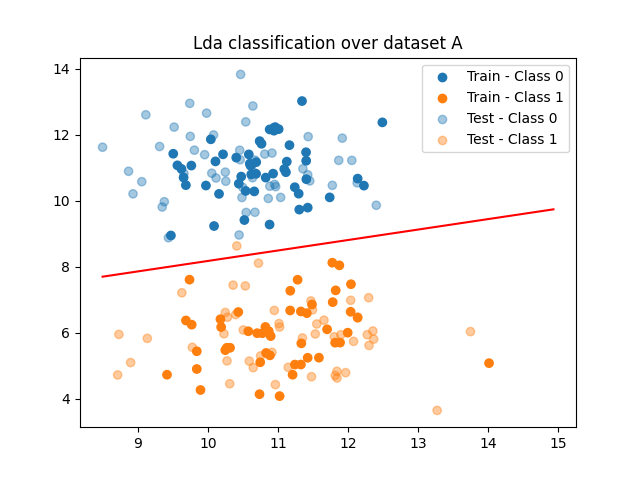
\includegraphics[width=\linewidth]{A_lda}
    \end{subfigure}
    \begin{subfigure}[b]{0.3\linewidth}
        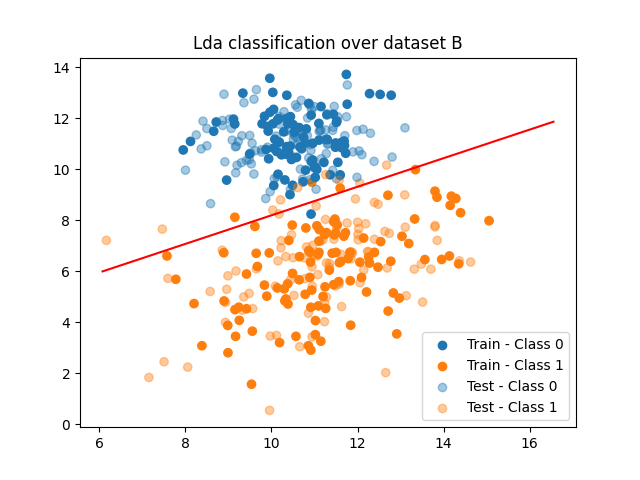
\includegraphics[width=\linewidth]{B_lda}
    \end{subfigure}
    \begin{subfigure}[b]{0.3\linewidth}
        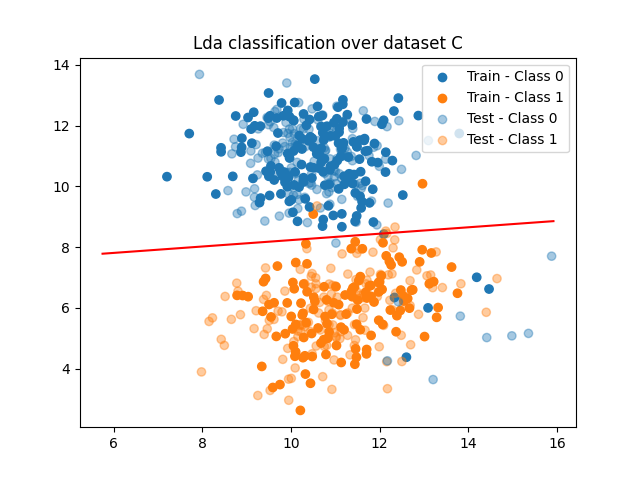
\includegraphics[width=\linewidth]{C_lda}
    \end{subfigure}
    \caption{Lda applied on the 3 datasets.}
    \label{fig:lda}
\end{figure}

\subsection{Logistic regression}

Implement logistic regression for an affine function $f(x)=w^Tx+b$ (do not forget the constant term).

\paragraph{a} Give the numerical values of the parameters learnt.\\
\vspace{10px}\\
Here we make the assumption that $y | x, w, b \sim \mathcal{B}(\sigma(w^Tx + b))$. \\
Let's $\theta^T = (b, w^T)$ and $x'^T = (1, x^T)$, then $y | x, \theta \sim  \mathcal{B}(\sigma(\theta^T x'))$.\\
The log-likelyhood is then:

\begin{equation*}
    \begin{aligned}
        L_{X, Y}(\theta) & = \sum_k \log p(y_k|x'_k, \theta)                                                      \\
                         & = \sum_k \log \mathcal{B}(y_k; \sigma(\theta^T x'_k))                                  \\
                         & = \sum_k y_k \log \sigma(\theta^T x'_k) + (1- y_k) \log (1 - \sigma(\theta^Tx'_k))     \\
                         & = - \sum_k y_k \log(1 + \exp(-\theta^T x'_k)) + (1 - y_k)\log(1 + \exp(\theta^T x'_k))
    \end{aligned}
\end{equation*}

Let $\widehat{\theta}$ a maximizer of $L_{X,Y}$ ($L$ is concave as $x \rightarrow \log(1 + \exp(\alpha x + \beta))$ is concave).

\begin{equation*}
    \nabla L_{X_Y}(\widehat\theta) = 0
\end{equation*}

And we can compute the gradient of $L$:
\begin{equation*}
    \begin{aligned}
        \nabla L_{X,Y}(\theta) & = \sum_k y_k \frac{\exp(-\theta^T x'_k)}{ 1 + \exp(-\theta^T x'_k)} x'_k - (1-y_k) \frac{\exp(\theta^T x'_k)}{ 1 + \exp(\theta^T x'_k)} x'_k \\
                               & = \sum_k \frac{y_k \exp(-\theta^T x'_k) - (1- y_k)}{ 1 + \exp(-\theta^T x'_k)} x'_k                                                          \\
                               & = \sum_k (y_k - \frac{1}{1 + \exp(-\theta^T x'_k)}) x'_k                                                                                     \\
                               & = \sum_k (y_k - \sigma(\theta^T x'_k)) x'_k
    \end{aligned}
\end{equation*}
The equation $\boxed{\nabla L_{X_Y}(\widehat\theta) = 0}$ is non-linear.
I will solve it using an already implemented algorithm for those kind of problems (with scipy). Which gives the following parameters:
\begin{tabular}{| c || c | c | c |}
    \hline
    $\mathbf{Dataset}$ & \multicolumn{2}{|c|}{$\mathbf{w}$} & $\mathbf{b}$           \\
    \hline
    A                  & 23.195                             & -59.613      & 264.416 \\
    \hline
    B                  & 1.842                              & -3.714       & 13.430  \\
    \hline
    C                  & -0.277                             & -1.914       & 18.807  \\
    \hline
\end{tabular}



\paragraph{b} Represent graphically the data as a cloud point in $\R^2$ as well as the line defined by the equation
\begin{equation*}
    p(y=1|x)=0.5
\end{equation*}
As before the equation of the line is:
\begin{equation*}
    \begin{aligned}w^Tx + b = 0
    \end{aligned}
\end{equation*}
The implementation can be found in the logistic.py file. In order to run the code you can use the command:
\begin{lstlisting}{bash}
    $ python exercise1.py --method logistic --data-directory /path/to/data
\end{lstlisting}

\begin{figure}[h!]
    \centering
    \begin{subfigure}[b]{0.3\linewidth}
        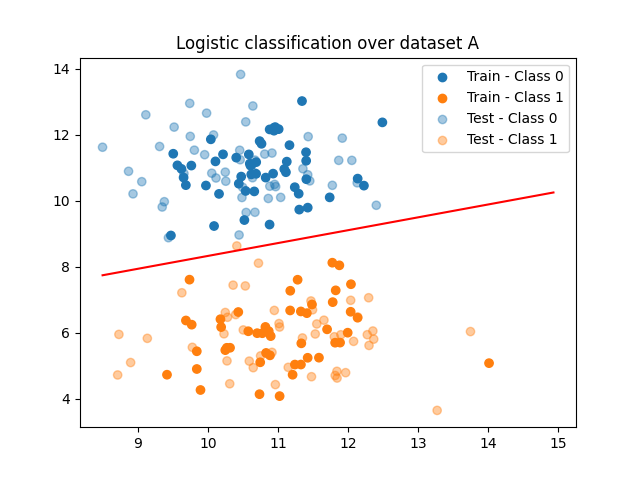
\includegraphics[width=\linewidth]{A_logistic}
    \end{subfigure}
    \begin{subfigure}[b]{0.3\linewidth}
        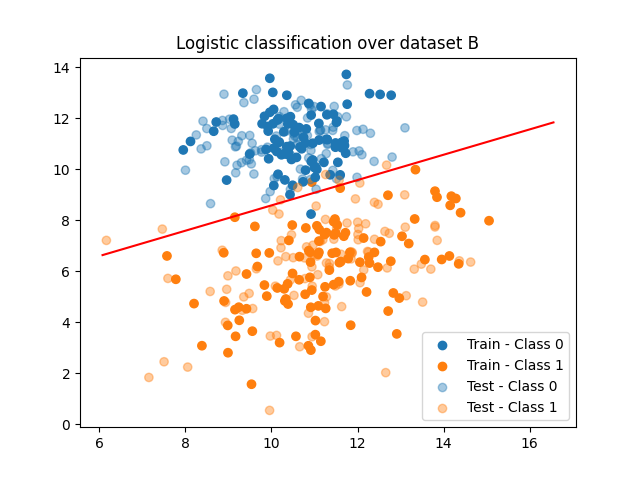
\includegraphics[width=\linewidth]{B_logistic}
    \end{subfigure}
    \begin{subfigure}[b]{0.3\linewidth}
        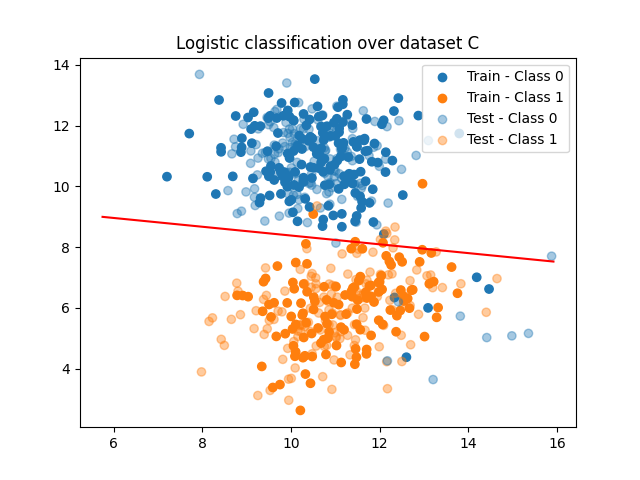
\includegraphics[width=\linewidth]{C_logistic}
    \end{subfigure}
    \caption{Logistic regression applied on the 3 datasets.}
    \label{fig:logistic}
\end{figure}

\subsection{Linear regression}
Consider class $y$ as a real valued variable taking the values $0$ and $1$ only. Implement linear regression
(for an affine function $f(x)=w^Tx+b)$ by solving the normal equations.

\paragraph{a} Provide the numerical values of the learnt parameters.\vspace{10px}\\
Let's use gaussian additive noise model (We will see that this will lead to the OLS problem):
$y = w^Tx + b + \epsilon$ where $\epsilon \sim \mathcal{N}(0, \alpha)$. The log-likelyhood is:
\begin{equation*}
    \begin{aligned}
        L_{X, Y}(w, b) & = \sum_k \log p(y_k | x_k, w, b)                           \\
                       & = \sum_k \log p(\epsilon = w^Tx + b - y_k | x_k, w, b)     \\
                       & = \sum_k \log \mathcal{N}(w^Tx + b - y_k; 0, 1)            \\
                       & = \text{cst} - \frac{1}{2\alpha} \sum_k (w^Tx + b - y_k)^2
    \end{aligned}
\end{equation*}\\
The maximization of the likelyhood gives:
\begin{equation*}
    \begin{aligned}
         & w, b \in \text{argmax } L_{X, Y}(w, b)                        \\
         & w, b \in \text{argmin} \sum_k \left(y_k - w^Tx_k - b\right)^2
    \end{aligned}
\end{equation*}\\
Maximizing the likelyhood is equivalent to the Ordinary Least Square problem.
Which can be written, using the previous notation $\theta^T = (b, w^T), x'^T_k = (1, x_k^T)$:
\begin{equation*}
    \begin{aligned}
         & \widehat\theta \in \text{argmin} \sum_k \left(y_k - \theta^Tx'_k\right)^2 \\
         & \widehat\theta \in \text{argmin} \norm{Y - X'\theta}_2^2
    \end{aligned}
\end{equation*}\\
One can see that if $\Ker(X') \neq {0}$ then the solution is not unique. (The solutions
then are $\widehat\theta + \Ker{X'}$, with $\widehat{\theta}$ a particular solution.)\\
Let's find a particular solution $\widehat\theta$: It is an extremum point of $\norm{Y - X'\theta}_2^2$ therefore we have
\begin{equation*}
    \begin{aligned}
        X'^T (Y - X'\widehat\theta) = 0              \\
        X'^T X' \widehat\theta = X'^T Y              \\
        \boxed{\widehat\theta = (X'^T X')^{+}X'^T Y} \\
    \end{aligned}
\end{equation*}\\
Using the Moore-Penrose inverse of $A$: $A^{+}$. I will directly use an implemented algorithm to compute the solution. (With numpy.)
Which gives the following parameters:
\begin{tabular}{| c || c | c | c |}
    \hline
    $\mathbf{Dataset}$ & \multicolumn{2}{|c|}{$\mathbf{w}$} & $\mathbf{b}$         \\
    \hline
    A                  & 0.056                              & -0.176       & 1.383 \\
    \hline
    B                  & 0.083                              & -0.148       & 0.882 \\
    \hline
    C                  & 0.017                              & -0.159       & 1.64  \\
    \hline
\end{tabular}

\paragraph{b.} Represent graphically the data as a point cloud in $\R^2$ as well as the line defined by the equation
\begin{equation*}
    p(y=1|x)=0.5
\end{equation*}
Let's add a small decision function to this equation so that it makes sense.
(Indeed in our current model: $p(y=1 | x) = 0$ as $y$ follows a normal distribution.) Let's instead consider $z = \mathds{1}_{\inter{0.5}{+\infty}}(y)$, and
now we can consider the line:

\begin{equation*}
    \begin{aligned}
        p(z=1|x) = 0.5                                       \\
        \Leftrightarrow p(y \ge 0.5|x) = 0.5                 \\
        \Leftrightarrow p(\epsilon \ge 0.5 - w^Tx - b) = 0.5 \\
        \Leftrightarrow w^Tx + b = 0.5
    \end{aligned}
\end{equation*}
The implementation can be found in the linear.py file. In order to run the code you can use the command:
\begin{lstlisting}{bash}
    $ python exercise1.py --method linear --data-directory /path/to/data
\end{lstlisting}

\begin{figure}[h!]
    \centering
    \begin{subfigure}[b]{0.3\linewidth}
        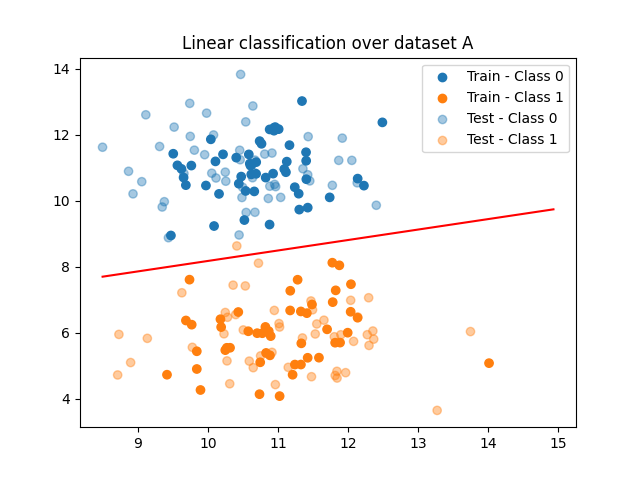
\includegraphics[width=\linewidth]{A_linear}
    \end{subfigure}
    \begin{subfigure}[b]{0.3\linewidth}
        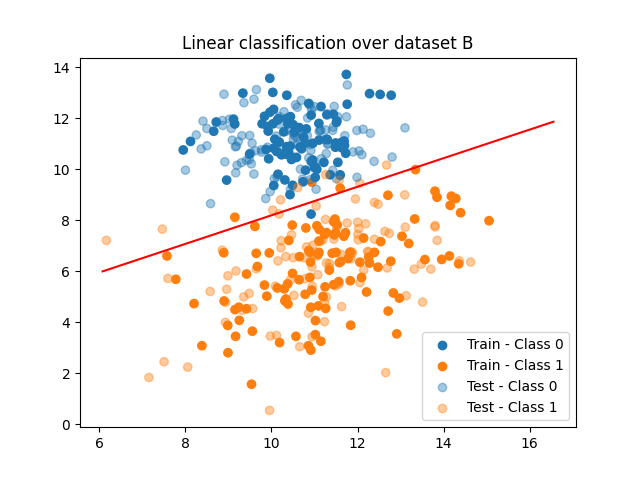
\includegraphics[width=\linewidth]{B_linear}
    \end{subfigure}
    \begin{subfigure}[b]{0.3\linewidth}
        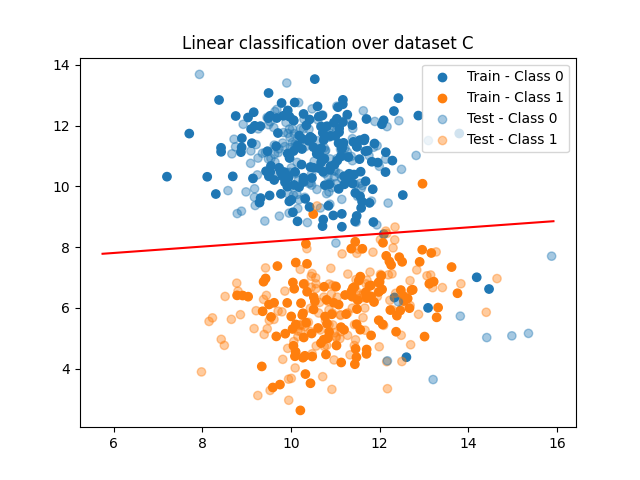
\includegraphics[width=\linewidth]{C_linear}
    \end{subfigure}
    \caption{Linear regression applied on the 3 datasets.}
    \label{fig:linear}
\end{figure}


\subsection{Application}
Data in the files testA, testB and testC are respectively drawn from the same distribution
as the data in the files trainA, trainB and trainC. Test the different models learnt from the corresponding training data on these test data.

\paragraph{a.} Compute for each model the misclassification error (i.e. the fraction of the data misclassified)
on the training data and compute it as well on the test data.\vspace{10px}

\begin{center}
    \begin{tabular}{| c || c | c || c | c || c | c |}
        \hline
        \multirow{2}{*}{$\mathbf{Dataset}$} & \multicolumn{2}{|c||}{$\mathbf{LDA}$} & \multicolumn{2}{|c|}{$\mathbf{Logistic}$} & \multicolumn{2}{|c|}{$\mathbf{Linear}$}                         \\
                                            & Train                                 & Test                                      & Train                                   & Test  & Train & Test  \\
        \hline
        A                                   & 0.0                                   & 0.01                                      & 0.0                                     & 0.01  & 0.0   & 0.01  \\
        \hline
        B                                   & 0.02                                  & 0.045                                     & 0.01                                    & 0.035 & 0.02  & 0.045 \\
        \hline
        C                                   & 0.027                                 & 0.04                                      & 0.03                                    & 0.047 & 0.27  & 0.4   \\
        \hline
    \end{tabular}
\end{center}

\paragraph{b.} Compare the performances of the different methods on the three datasets. Is the misclassification error larger, smaller,
or similar on the training and test data? Why? Which methods yield very similar/dissimilar results? Which methods yield the best
results on the different datasets ? Provide an interpretation.\vspace{10px}

Firstly models make more errors on the test sets than on the train sets which is totally expected. Indeed models are designed to separate the train sets.
(With a reasonable hope that it will generalize to similar test data.)

Secondly the Linear Regression and the LDA have very similar results over all the datasets (They provide very similar separation line.). The
Logistic Regression is a little bit different from them. For the dataset A (the simplest one, where data are the most linearly separable),
all the methods perform equivalently. For the dataset B Logistic Regression seems to outperform the others. And for the dataset C,
it's the LDA and the Linear Regression that perform best.

We could have guessed that LDA would not have been the best one on dataset B because our statistical model can not fit the data: It seems indeed that
the two classes have been generated through two gaussians with different covariance matrixes (whereas LDA assume that they are equals).

\section{Gaussian mixture models and EM}
We consider the following Gaussian mixture model (GMM) for multivariate data:
\begin{equation*}
    X_i \sim \sum_{k=1}^K \pi_k \mathcal{N}(\mu_k, \Sigma_k)
\end{equation*}
with $\pi_k \in \inter{0}{1}$, $\sum_k \pi_k = 1$ and $x \in \R^p$. We are provided with a realisation $(x_1,\dots,x_n)$ of a random sample of size n.

\subsection{Math}

Let's introduce the hidden random variables $Z_i \in \R^K$ such that $(X_i, Z_i)_i$ are independent and identically distributed and:
\begin{equation*}
    \begin{aligned}
         & Z_i \sim \mathcal{M}(1, \pi)                      & (\Rightarrow p(Z_i = e_k) = \pi_k) \\
         & X_i | Z_i = e_k \sim \mathcal{N}(\mu_k, \Sigma_k) &
    \end{aligned}
\end{equation*}
One can see then that $p(x_i |\theta) = \sum_k p(x_i, Z_i=e_k |\theta) = \sum_k \pi_k \mathcal{N}(\mu_k, \Sigma_k)$. It's the same statistical model.\\
(Note: $(e_k)_{k \in \Inter{1}{K}}$ is the canonical basis of $\R^K$: ${e_k}_i = \delta_{ik}$)
\vspace{10px}\\
In my notation, $p$ is a density function which refers to many different random variables knowing $\theta$: one of the $X_i$, $Z_i$, $(X_i, Z_i)$,
for $i \in \Inter{1}{n}$ or even $(X_i)_{i \in \Inter{1}{n}}$, $(Z_i)_{i \in \Inter{1}{n}}$ or $(X_i, Z_i)_{i \in \Inter{1}{n}}$. (I will be as clear
as possible to differentiate them.)
\vspace{10px}\\
Let $(Y_i)_i$ $n$ random variables over $\R^K$ of distribution $R$.
$R$ is either the density function of one of the $Y_i$ or of $(Y_i)_{i \in \Inter{1}{n}}$.\\
The log-likelyhood of $\theta = {(\pi_k, \mu_k, \Sigma_k)}_k$ can be decompose using this distribution $R$:
\begin{equation*}
    \begin{aligned}
        L_X(\theta) & = \log p(X | \theta)                                                                                                                     &                                            \\
                    & = \sum_{Y \in \R^{n\times K}} R(Y) \log p(X | \theta)                                                                                    & \text{(The sum of $R(Y)$ is equal to one)} \\
                    & = \sum_{Y \in \R^{n\times K}} R(Y) \log \frac{p(X | \theta)p((Z_i)_i=Y|X,\theta)}{p((Z_i)_i=Y|X, \theta)}                                &                                            \\
                    & = \sum_{Y \in \R^{n\times K}} R(Y) \log \frac{p(X, Y | \theta)}{p(Y|X, \theta)}                                                          & \text{(Bayes formula)}                     \\
                    & = \sum_{Y \in \R^{n\times K}} R(Y) \log \frac{p(X, Y | \theta)R(Y)}{p(Y|X, \theta)R(Y)}                                                  &                                            \\
                    & = \sum_{Y \in \R^{n\times K}} R(Y) \log \frac{p(X, Y | \theta)}{R(Y)} - \sum_{Y\in \R^{n\times K}} R(Y) \log \frac{p(Y|X, \theta)}{R(Y)} &                                            \\
                    & = \mathcal{L}_X(R, \theta) + \text{KL}(R,\, p_{Z|X, \theta})
    \end{aligned}
\end{equation*}
The EM algorithm uses this decomposition in two steps: \begin{itemize}
    \item (E): Given $\theta$ choose $R$ that maximizes $\mathcal{L}_X(., \theta)$ (As $L$ is independent of $R$, this $R$ will also minimize KL up to $0$)
    \item (M): Given $R$ find $\theta$ that maximizes $\mathcal{L}_X(R, .)$
    \item Go back to (E)
\end{itemize}
It will maximize the likelyhood:
indeed, given a $\theta^l$, the computation of $R^{l+1}$ is such that $L_X(\theta^l) = \mathcal{L}_X(R^{l+1}, \theta^l) + 0$, then we compute
$\theta^{l+1}$ maxizing $\mathcal{L}_X$ and therefore $\mathcal{L}_X(R^{l+1}, \theta^{l+1}) \ge \mathcal{L}_X(R^{l+1}, \theta^l)$. Then
with the computation of $R^{l+2}$ maximizing $\mathcal{L}_X$ and minimizing KL we have:

\begin{equation*}
    \begin{aligned}
        L_X(\theta^{l+1}) & = \mathcal{L}_X(R^{l+2}, \theta^{l+1})   & \text{(Because $R^{l+2}$ minimizes KL up to $0$)}                     \\
                          & \ge \mathcal{L}_X(R^{l+1}, \theta^{l+1}) & \text{(Because $R^{l+2}$ maximizes $\mathcal{L}_X(., \theta^{l+1})$)} \\
                          & \ge \mathcal{L}_X(R^{l+1}, \theta^{l})   & \text{(Because $\theta^{l+1}$ maximizes $\mathcal{L}_X(R^{l+1}, .)$)} \\
                          & = L_X(\theta^l)
    \end{aligned}
\end{equation*}


\paragraph{Resolve E step} Let $\theta = {(\pi_k, \mu_k, \Sigma_k)}_k$ given.\vspace{10px}\\
In order to maximize $\mathcal{L}_X$ w.r.t $R$ we have to choose $R$ such that $\text{KL}(R,\, p_{Z|X, \theta}) = 0$. Let $Y = (y_i)_i \in \R^{n\times p}$:
\begin{equation*}
    \begin{aligned}
        R(Y)                       & = p(Y | X, \theta)                                                                                       & \text{(In order to have KL $= 0$)}                                                                                              \\
                                   & = \prod_i p(y_i|x_i, \theta)                                                                             & \text{($(X_i,Z_i)_i$ iid})                                                                                                      \\
                                   & = \prod_i \frac{p(y_i, x_i|\theta)}{p(x_i|\theta)}                                                       & \text{(Bayes formula)}                                                                                                          \\
                                   & = \prod_i \frac{p(x_i|y_i, \theta)p(y_i|\theta)}{\sum_{l=1}^K p(Z_i = e_l|\theta)p(x_i|Z_i=e_l, \theta)} & \text{(Bayes again)}                                                                                                            \\
                                   & = \vast\{
        \begin{aligned}
             & 0                                                                                                                                    &  & \text{If } \exists i \in \Inter{1}{n}, \forall k \in \Inter{1}{K}, y_i \neq e_k \\
             & \prod_i \frac{\prod_k \left(\pi_k\mathcal{N}(x_i, \mu_k, \Sigma_k)\right)^{{y_i}_k}}{\sum_l \pi_l \mathcal{N}(x_i, \mu_l, \Sigma_l)} &  & \text{Otherwise}                                                                \\
        \end{aligned} &                                                                                                                                                                                                                                            \\
                                   & = \vast\{
        \begin{aligned}
             & \prod_i \prod_k \left(\frac{\pi_k\mathcal{N}(x_i, \mu_k, \Sigma_k)}{\sum_l \pi_l \mathcal{N}(x_i, \mu_l, \Sigma_l)}\right)^{{y_i}_k} &  & \text{If } \forall i, y_i \in \set{e_k, k\in\Inter{1}{K}} \\
             & 0                                                                                                                                    &  & \text{Otherwise}                                          \\
        \end{aligned} &                                                                                                                                                                                                                                            \\
                                   & \boxed{= \prod_i \mathcal{M}(y_i; 1, \tau_i)}                                                            & \boxed{\text{with } {\tau_i}_k = \frac{\pi_k\mathcal{N}(x_i, \mu_k, \Sigma_k)}{\sum_l \pi_l \mathcal{N}(x_i, \mu_l, \Sigma_l)}} \\
    \end{aligned}
\end{equation*}

\paragraph{Resolve M step} Let $R = \prod_i \mathcal{M}(1, \tau_i)$ given.\vspace{10px}
\begin{equation*}
    \begin{aligned}
        \widehat\theta & \in \text{argmax}_{\theta} \mathcal{L}_X(R, \theta)                                                      &                                                              \\
        \widehat\theta & \in \text{argmax}_{\theta} \sum_Y R(Y) \log \frac{p(X, Y | \theta)}{R(Y)}                                &                                                              \\
        \widehat\theta & \in \text{argmax}_{\theta} \sum_Y R(Y) \log p(X, Y | \theta)                                             & (\sum_{Y} R(Y) \log R(Y) \text{ is a constant w.r.t }\theta) \\
        \widehat\theta & \in \text{argmax}_\theta \sum_Y R(Y) \sum_i \log p(x_i | y_i | \theta) p(y_i|\theta)                     & \text{(iid + bayes formula)}                                 \\
        \widehat\theta & \in \text{argmax}_\theta \sum_Y R(Y) \sum_i \sum_k {y_i}_k \log \pi_k \mathcal{N}(x_i, \mu_k, \Sigma_k)  & (Z_i \sim \mathcal{M}(1, \pi))                               \\
        \widehat\theta & \in \text{argmax}_\theta \sum_i \sum_k \log (\pi_k\mathcal{N}(x_i, \mu_k, \Sigma_k)) \sum_Y R(Y) {y_i}_k &                                                              \\
        \widehat\theta & \in \text{argmax}_\theta \sum_i \sum_k {\tau_i}_k \log \pi_k \mathcal{N}(x_i, \mu_k, \Sigma_k)           & (\sum_Y R(Y) {y_i}_k = \E_{Y \sim R}[{y_i}_k] = {\tau_i}_k)
    \end{aligned}
\end{equation*}
Let's first compute $\widehat\pi$. One can see that the problem can be solved separately for $\pi$ and for $\mu, \Sigma$.
And we have also the condition $\sum_k pi_k = 1$: Thus the problem for $\pi$ is:

\begin{equation*}
    (P):\;\;\;
    \begin{aligned}
         & \widehat{\pi} \in \text{argmax}_\pi &  & \sum_i \sum_k {\tau_i}_k \log \pi_k \\
         & \text{subject to}                   &  & \sum_k \pi_k = 1                    \\
    \end{aligned}
    \;\;\Leftrightarrow\;\;
    \begin{aligned}
         & \widehat{\pi} \in \text{argmin}_\pi &  & - \sum_i \sum_k {\tau_i}_k \log \pi_k \\
         & \text{subject to}                   &  & \sum_k \pi_k - 1 = 0                  \\
    \end{aligned}
\end{equation*}
The lagrangian of the problem is:
\begin{equation*}
    \begin{aligned}
        \mathcal{L}(\pi, \nu) & = - \sum_i \sum_k {\tau_i}_k \log \pi_k + \nu (\sum_k \pi_k -1)       \\
                              & =  \sum_k \left[ \nu \pi_k - \sum_i \tau_{ik} \log \pi_k\right] - \nu
    \end{aligned}
\end{equation*}
And the dual function is:
\begin{equation*}
    \begin{aligned}
        g(\nu) & = \inf_\pi L(\pi, \nu)                                                             \\
               & =  \sum_k \inf_{\pi_k} \left[ \nu \pi_k - \sum_i \tau_{ik} \log \pi_k\right] - \nu \\
    \end{aligned}
\end{equation*}
Here either $\nu \le 0$ and the infimum over any $\pi_k$ is $-\infty$ (taking $\pi \rightarrow +\infty$), or $\nu > 0$ and
we can derivate the function w.r.t $\pi_k$ (twice to show that this is convex. And once to find the optimum $\pi_k$):
$\pi_k = \frac{1}{\nu} \sum_i \tau_{ik}$.\\
g can therefore be written:
\begin{equation*}
    \begin{aligned}
        g(\nu) & = \vast\{
        \begin{aligned}
             & -\infty                                                                                                          & \text{If } \nu \le 0 \\
             & \sum_k \left[ \sum_i \tau_{ik} + \sum_i \tau_{ik} \log\nu - \sum_i \tau_{ik} \log \sum_i \tau_{ik} \right] - \nu & \text{Otherwise}     \\
        \end{aligned} \\
               & = \vast\{
        \begin{aligned}
             & -\infty                                                             & \text{If } \nu \le 0 \\
             & n + n \log\nu - \nu - \sum_i \sum_k \tau_{ik} \log \sum_i \tau_{ik} & \text{Otherwise}     \\
        \end{aligned} \\
    \end{aligned}
\end{equation*}
The dual problem is therefore equivalent to:
\begin{equation*}
    (D):\;\;\;
    \begin{aligned}
         & \widehat{\nu} \in \text{argmax}_\nu &  & n \log\nu - \nu + \text{cst} \\
    \end{aligned}
\end{equation*}
The solution of the dual is trivial (we did it before: derived $a \log\nu - b\nu$): $\widehat{\nu} = n$.\\
Then as strong duality holds (from slater's condition), $\widehat\pi \in \text{argmin}_\pi \mathcal{L}(\pi, \widehat\nu)$:

\begin{equation*}
    \boxed{\widehat{\pi}_k = \frac{1}{\widehat{\nu}} \sum_i \tau_{ik} = \frac{n_k}{n} \;\;\;\;\;\;\;\;\;\;\text{(With $n_k = \sum_i \tau_{ik}$)}}
\end{equation*}
Then we can focus on the the other parameters, $\mu$ and $\Sigma$, here as there is no condition over them we will only use that they are an
extremum point of a differentiable function:

\begin{equation*}
    \widehat\mu, \widehat\Sigma \in \text{argmax}_{\mu, \Sigma}\;\; \text{cst} - \frac{1}{2} \sum_k n_k \log|\Sigma_k| - \frac{1}{2} \sum_i \sum_k \tau_{ik} (x_i - \mu_k)^T \Sigma_k^{-1} (x_i - \mu_k)
\end{equation*}
And as for exercise 1.1 we can use the gradient to find our parameters. Let's focus on $\widehat\mu_k$:

\begin{equation*}
    \begin{aligned}
        \sum_i \tau_{ik} \widehat\Sigma_k^{-1} (x_i - \widehat\mu_k) = 0 \\
        \sum_i \tau_{ik} x_i - \sum_i \tau_{ik} \widehat\mu_k = 0        \\
        \boxed{\widehat\mu_k = \frac{1}{n_k}\sum_i \tau_{ik} x_i}        \\
    \end{aligned}
\end{equation*}
And for $\widehat\Sigma$:
\begin{equation*}
    \begin{aligned}
        -\frac{n_k}{2} \widehat\Sigma_k^{-1} + \frac{1}{2}\widehat\Sigma_k^{-1} \sum_i \tau_{ik}  (x_i - \widehat\mu_k)(x_i - \widehat\mu_k)^T \widehat\Sigma_k^{-1} & = 0 \\
        \widehat\Sigma_k - \frac{1}{n_k} \sum_i \tau_{ik}  (x_i - \widehat\mu_k)(x_i - \widehat\mu_k)^T                                                              & =0  \\
        \boxed{\widehat\Sigma_k = \frac{1}{n_k}\sum_i \tau_{ik} (x_i - \widehat\mu_k)(x_i - \widehat\mu_k)^T}                                                        &     \\
    \end{aligned}
\end{equation*}
This ends the M-Step.

\subsection{Implementation}

For the implementation I will use the already implemented KMeans of Scikit-learn to initialized $\tau$. (I will also provide a handmade
random initialization of $\tau$). The rest does only rely on numpy array and their computation of inverse/determinant.

The GMM is implemented in the file gmm.py. In order to run the code you can use the command:
\begin{lstlisting}{bash}
    # For GMM on the 2D datas:
    $ python exercise2.py --visual --data-directory /path/to/data
    # For GMM on the decathlon dataset:
    $ python exercise2.py --data-directory /path/to/data --clusters 3 --init random
\end{lstlisting}

\subsection{Application}
\paragraph{On previous datasets.} Let's first focus on the previous dataset.\vspace*{10px}\\
The EM algorithm works very well in this case. It converges fast, in around 10 iterations with a kmeans initialization, and around 50 iterations
with a random one. Even if the algorithm is unsupervised, it will learn a better classifier for the previous datasets than the 3 methods in part 1:

\begin{center}
    \begin{tabular}{| c || c | c |}
        \hline
        \multirow{2}{*}{$\mathbf{Dataset}$} & \multicolumn{2}{|c|}{$\mathbf{GMM}$}         \\
                                            & Train                                & Test  \\
        \hline
        A                                   & 0.0                                  & 0.01  \\
        \hline
        B                                   & 0.015                                & 0.025 \\
        \hline
        C                                   & 0.027                                & 0.033 \\
        \hline
    \end{tabular}
\end{center}
We could have expected those kind of results because it models much better the datasets that we have here. The GMM classifier with 2 classes that we get is
a non-linear classifier:
\begin{figure}[h!]
    \centering
    \begin{subfigure}[b]{0.3\linewidth}
        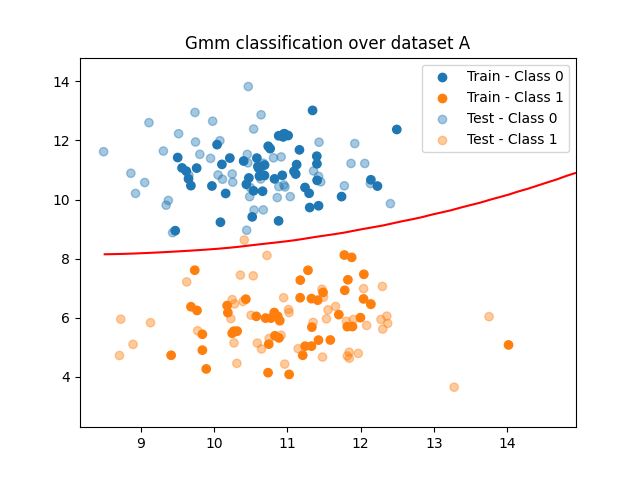
\includegraphics[width=\linewidth]{A_gmm}
    \end{subfigure}
    \begin{subfigure}[b]{0.3\linewidth}
        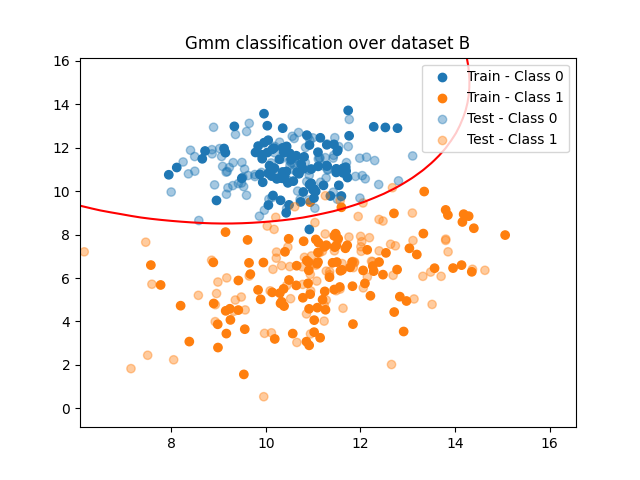
\includegraphics[width=\linewidth]{B_gmm}
    \end{subfigure}
    \begin{subfigure}[b]{0.3\linewidth}
        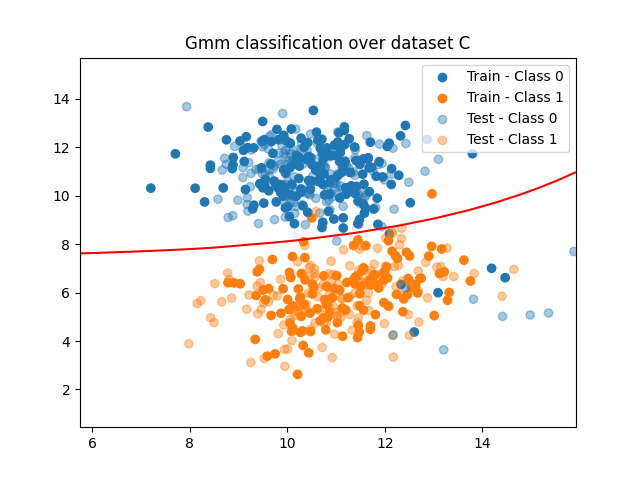
\includegraphics[width=\linewidth]{C_gmm}
    \end{subfigure}
    \caption{Gaussian Mixture Model applied on the 3 datasets.}
    \label{fig:gmm}
\end{figure}

\paragraph{On decathlon dataset.} Use your EM algorithm to analyse the decathlon data set and to look for $K=3$ clusters.
Interpret the results. The data used here refer to athletes’ performance during decathlon events.
\vspace*{10px}\\
In this case I've faced lots of issues:

First I had to ensure that $\Sigma$ were all positive matrixes (by addding a regularization to each diagonal of them.)

Second, the convergence can be tricky to have. And depends a lot of initialization. With kmeans log-likelihood often never changed with the EM algorithm
(It seems that the algorithm is stuck with the initialization of kmeans and can't improve it). And with random initialization, it's very unstable.
So I try to do multiple EMs and take the best one w.r.t the likelyhood. But still the results have lots of variability.
\vspace*{10px}\\
This being said it's quite difficult to interpret the results with a high confidence. It would be expected that the EM finds group of athletes
that performs well in the same fields. For instance we could have expected a group of runners, a group of throwers and a group of jumpers.

Sadly even if sometimes clusters seems to have some meanings (E.g. best performers on 1500m and 400m are very often together), I think
that with the variability of the results it's more likely that such an obvious clustering does not exist.

\end{document}
